\documentclass{article}\usepackage[]{graphicx}\usepackage[]{color}
%% maxwidth is the original width if it is less than linewidth
%% otherwise use linewidth (to make sure the graphics do not exceed the margin)
\makeatletter
\def\maxwidth{ %
  \ifdim\Gin@nat@width>\linewidth
    \linewidth
  \else
    \Gin@nat@width
  \fi
}
\makeatother

\definecolor{fgcolor}{rgb}{0.345, 0.345, 0.345}
\newcommand{\hlnum}[1]{\textcolor[rgb]{0.686,0.059,0.569}{#1}}%
\newcommand{\hlstr}[1]{\textcolor[rgb]{0.192,0.494,0.8}{#1}}%
\newcommand{\hlcom}[1]{\textcolor[rgb]{0.678,0.584,0.686}{\textit{#1}}}%
\newcommand{\hlopt}[1]{\textcolor[rgb]{0,0,0}{#1}}%
\newcommand{\hlstd}[1]{\textcolor[rgb]{0.345,0.345,0.345}{#1}}%
\newcommand{\hlkwa}[1]{\textcolor[rgb]{0.161,0.373,0.58}{\textbf{#1}}}%
\newcommand{\hlkwb}[1]{\textcolor[rgb]{0.69,0.353,0.396}{#1}}%
\newcommand{\hlkwc}[1]{\textcolor[rgb]{0.333,0.667,0.333}{#1}}%
\newcommand{\hlkwd}[1]{\textcolor[rgb]{0.737,0.353,0.396}{\textbf{#1}}}%

\usepackage{framed}
\makeatletter
\newenvironment{kframe}{%
 \def\at@end@of@kframe{}%
 \ifinner\ifhmode%
  \def\at@end@of@kframe{\end{minipage}}%
  \begin{minipage}{\columnwidth}%
 \fi\fi%
 \def\FrameCommand##1{\hskip\@totalleftmargin \hskip-\fboxsep
 \colorbox{shadecolor}{##1}\hskip-\fboxsep
     % There is no \\@totalrightmargin, so:
     \hskip-\linewidth \hskip-\@totalleftmargin \hskip\columnwidth}%
 \MakeFramed {\advance\hsize-\width
   \@totalleftmargin\z@ \linewidth\hsize
   \@setminipage}}%
 {\par\unskip\endMakeFramed%
 \at@end@of@kframe}
\makeatother

\definecolor{shadecolor}{rgb}{.97, .97, .97}
\definecolor{messagecolor}{rgb}{0, 0, 0}
\definecolor{warningcolor}{rgb}{1, 0, 1}
\definecolor{errorcolor}{rgb}{1, 0, 0}
\newenvironment{knitrout}{}{} % an empty environment to be redefined in TeX

\usepackage{alltt}
\usepackage[letterpaper, portrait, margin=1in]{geometry}
\usepackage{amsmath}
\usepackage{hyperref}

\title{MATH 680 - Assignment \#3}
\author{Kevin McGregor}
\date{November 11th, 2015}
\IfFileExists{upquote.sty}{\usepackage{upquote}}{}
\begin{document}
\maketitle

%Beta tilde
\newcommand{\tb}{\tilde{\beta}}
\newcommand{\sign}{\mbox{sign}}

\section*{Question 1}
\subsection*{(a)}
We know that the least squares criterion is a convex function.  Also, if we were to find the gradient of the objective function, the $k^{th}$ element of the second term in the objective function would be:
\begin{eqnarray*}
  \frac{\partial}{\partial\tb_k} \left( \frac{\lambda}{\alpha} \sum_{j=1}^{p-1} |\tb_k|^\alpha \right) &=& \lambda |\tb_k|^{\alpha-1}\sign(\tb_k),
\end{eqnarray*}
if $\tb_k \neq 0$.  Then the second partial derivative gives us:
\begin{eqnarray*}
  \frac{\partial^2}{\partial\tb_k^2} \left( \frac{\lambda}{\alpha} \sum_{j=1}^{p-1} |\tb_k|^\alpha \right) &=& \lambda \sign^2(\tb_k)(\alpha-1) |\tb_k|^{\alpha-2} \\
        &\geq& 0,
\end{eqnarray*}
if $\alpha \geq 1$ and $\tb_k \neq 0$.  Also, since the penalty term in the objective function is greater than or equal to zero, we know that $\tb_k$ is a global minimum with respect to the $k^{th}$ element.  Therefore, the penalty term is a convex function.  Since both terms in the objective function are convex, the objective function is, itself, convex.

\subsection*{(b)}
Since the first derivative involves the power $\alpha-1$, we can see that the function is differentiable for $\alpha>1$.  But the second derivative involves the power $\alpha-2$, and is therefore not twice differentiable for $\alpha<2$ at zero.

\subsection*{(c)}
\emph{See R code for this function in 'bridgeReg.R'.}

\subsection*{(d)}
Testing for the \emph{bridgeReg} function can be found in 'a3\_q1d.R'.  The gradient at the returned value is, indeed approximately zero.

\section*{Question 2}
\subsection*{(a)}
Let $\eta_i=\mbox{ilogit}(e^{x_i^\top\beta})$. The objective function is proportional to:
\begin{eqnarray*}
 f(\beta) &=& -\sum_{i=1}^n n_i y_i \log\eta_i - \sum_{i=1}^n(\eta_i-n_i y_i)\log(1-\eta_i) + \frac{\lambda}{\alpha}\sum_{j=2}^p |\beta_j|^\alpha \\
 &=& -\sum_{i=1}^n n_i y_i \log\left(\frac{\eta_i}{1-\eta_i}\right) - \sum_{i=1}^n\eta_i\log(1-\eta_i) + \frac{\lambda}{\alpha}\sum_{j=2}^p |\beta_j|^\alpha
\end{eqnarray*}
Then the gradient is:
\begin{eqnarray*}
 \nabla f(\beta) &=& -\sum_{i=1}^n n_i y_i x_i  + \sum_{i=1}^n \frac{n_i x_i \exp(x_i^\top \beta)}{1+\exp(x_i^\top \beta}) + \lambda \left( \begin{array}{c}
 0 \\
\mbox{sign}(\beta_1) |\beta_2|^{\alpha-1}  \\
\vdots  \\
\mbox{sign}(\beta_p) |\beta_p|^{\alpha-1}  \end{array} \right) \\
&=& \sum_{i=1}^n n_i(\eta_i-y_i)x_i + \lambda \left( \begin{array}{c}
 0 \\
\mbox{sign}(\beta_1) |\beta_2|^{\alpha-1}  \\
\vdots  \\
\mbox{sign}(\beta_p) |\beta_p|^{\alpha-1}  \end{array} \right).
\end{eqnarray*}
Similarly, the second derivative is:
\begin{eqnarray*}
 \nabla^2 f(\beta) &=& \sum_{i=1}^n n_i(x_i\eta_i-x_i\eta_i^2)x_i^\top + \lambda(\alpha-1) \left( \begin{array}{cccc}
 0 & 0 & 0 & 0\\
 0 & \mbox{sign}(\beta_1) |\beta_2|^{\alpha-1} & 0 & 0  \\
 \vdots & & \ddots & \vdots \\
 0 & 0 & 0 & \mbox{sign}(\beta_p) |\beta_p|^{\alpha-1}  \end{array} \right) \\
\end{eqnarray*}
Since $\nabla^2 f(\beta)$ is positive definite, the function is strictly convex.

\subsection*{(b)}
\emph{The code for this question can be found in the file "bridgeLogistic.R"}.  I use the MM algorithm.  I will use the majorization function for the penalty term as seen in the first question of this assignment.  I will combine this with the second-order Taylor expansion for the negative log-likelihood term to find an overall majorization function:
\begin{eqnarray*}
 g(\beta|\bar{\beta}) &=& \left( X^\top[\tilde{n}\circ(\tilde{\eta}-y)] \right)(\beta-\bar{\beta}) + \frac{1}{2}\frac{\max(\tilde{n})}{4}(\beta-\bar{\beta})^\top(\beta-\bar{\beta}) + \frac{\lambda}{\alpha} \sum_{j=2}^p \left[|\bar{\beta}_j| + \frac{\alpha}{2}|\bar{\beta}_j|^{\alpha-2}\{\beta_j^2 - \bar{\beta}_j^2\} \right]
\end{eqnarray*}
because the term $\eta(1-\eta)$ appears in the second derivative, and is less than or equal to $1/4$ when $\eta \in (0,1)$.  Minimizing this majorization function gives us:

\begin{eqnarray*}
 \left(\frac{\max{\tilde{n}}}{4}X^\top X + \lambda M\right)\beta &=& - \left( X^\top[\tilde{n}\circ(\tilde{\eta}-y)] \right)
\end{eqnarray*}
The algorithm proceeds by iteratively resolving this system until convergence.

\subsection*{(c)}
The code for testing the bridge-penalized logistic regression function can be found in 'a3\_q2c.R'.  Unfortunatly, there is still something wrong with the code, as the returned estimate does not set the gradient to the zero vector.

\section*{Question 3}
\subsection*{(a)}
\emph{The code for this question can be seen in the file 'mixtureEM.R', under the function 'mixtureEM'.}

\subsection*{(b)}
\emph{The code for this question can be seen in the file 'mixtureEM.R', under the function 'mixtureEM\_csig'.}
We start by looking at the log-likelihood:
\begin{eqnarray*}
 l(\theta) &=& -\left[ \sum_{i=1}^n \log \left\{ \sum_{y=1}^C \phi(x_i;\mu_y,\Sigma)\pi_y \right\} \right].
\end{eqnarray*}
Then the expectation step involves the following quantity:
\begin{eqnarray*}
 q(\theta|\theta^{(k)}) &=& -\sum_{i=1}^n \sum_{y=1}^C \log \left\{ \phi(x_i;\mu_y,\Sigma)\pi_y \right\} \frac{\phi(x_i;\mu_y,\Sigma)\pi_y}{\sum_{j=1}^C \phi(x_i;\mu_j,\Sigma)\pi_y} \\
 &=& -\sum_{i=1}^n \sum_{y=1}^C  \left\{ -\frac{1}{2}(x_i-\mu_y)^\top\Sigma^{-1}(x_i-\mu_y) - \log((2\pi)^{p/2} |\Sigma^{-1}|^{-1/2} ) \right\} \gamma(z_{iy}),
\end{eqnarray*}
and we differentiate with respect to $\Sigma^{-1}$ to obtain:
\begin{eqnarray*}
 \frac{\partial q(\theta|\theta^{(k)})}{\partial\Sigma^{-1}} &=& -\sum_{i=1}^n \sum_{y=1}^C  \left\{ -\frac{1}{2}(x_i-\mu_y)^\top(x_i-\mu_y) + \frac{1}{2}\Sigma \right\} \gamma(z_{iy}).
\end{eqnarray*}
Setting $\frac{\partial q(\theta|\theta^{(k)})}{\partial\Sigma^{-1}}=0$ results in:

\begin{eqnarray*}
\sum_{i=1}^n \sum_{y=1}^C (x_i-\mu_y)^\top(x_i-\mu_y)\gamma(z_{iy}) &=& \Sigma \sum_{i=1}^n \sum_{y=1}^C \gamma(z_{iy}) \\
\Sigma &=& \frac{1}{\sum_{y=1}^{C}N_y} \sum_{i=1}^n \sum_{y=1}^C (x_i-\mu_y)^\top(x_i-\mu_y)\gamma(z_{iy}).
\end{eqnarray*}

Since, the other parameters have not changed from part (a), their derivatives have not changed and therefore their estimates for the next iteration have not changed either:
\begin{eqnarray*}
 N_y=\Sigma_{y=1}^{N}\gamma(z_{iy}), & \mu_y=\frac{1}{N_y}\Sigma_{y=1}^{N}\gamma(z_{iy})x_i, & \pi_y=\frac{N_y}{N}.
\end{eqnarray*}

\subsection*{(c)}
I chose the Abalone dataset to test the fuctions \url{https://archive.ics.uci.edu/ml/datasets/Abalone}.  Since there were over 4000 observations available, I took a random sample of 500 on which to test my code.  The three classifications are "Male", "Female", and "Infant".  The two variables I used in the algorithm were the length and diameter of the abalone.


\begin{knitrout}
\definecolor{shadecolor}{rgb}{0.969, 0.969, 0.969}\color{fgcolor}\begin{figure}
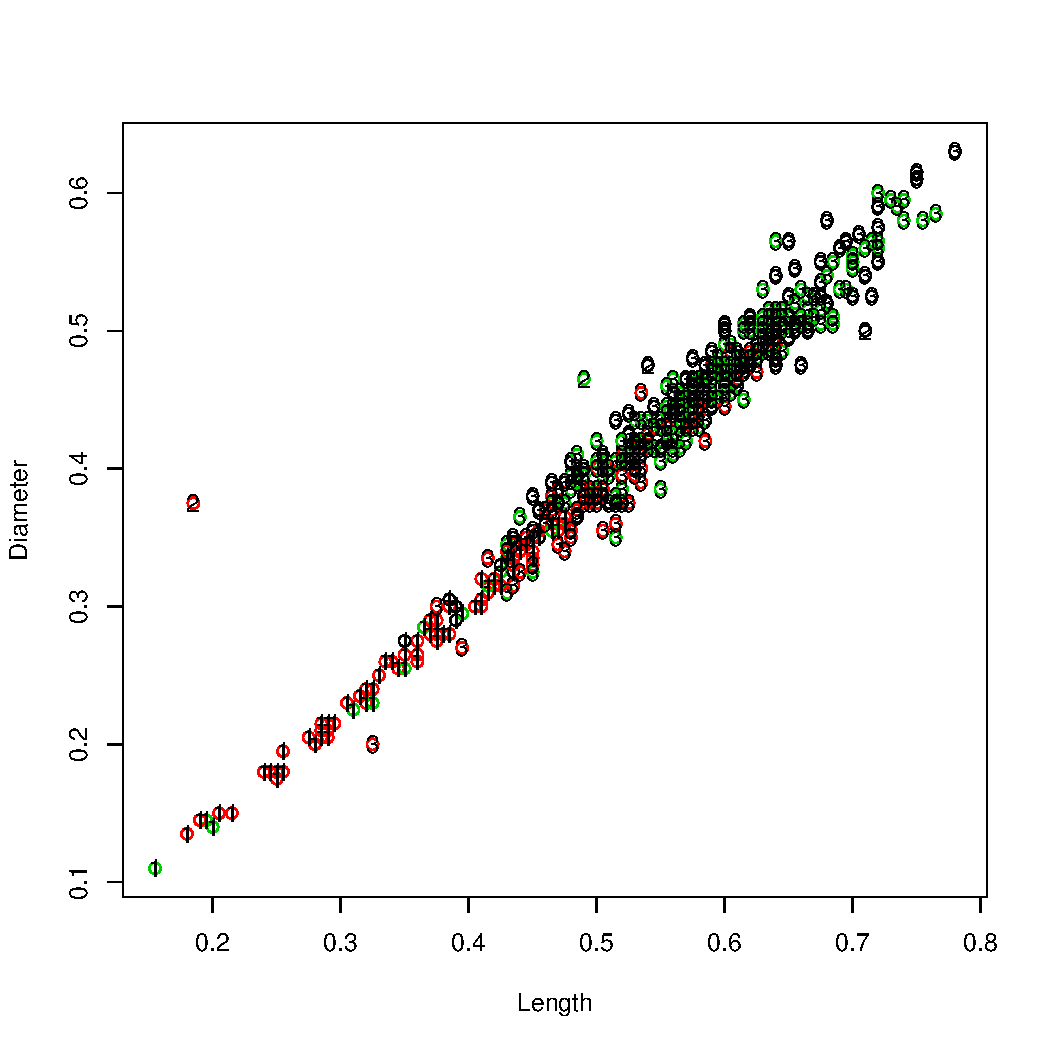
\includegraphics[width=\maxwidth]{figure/em_plot1-1} \caption[Classification of abalone based on length and diameter]{Classification of abalone based on length and diameter.  The algorithm used assumes the covariance matrix differs between the three categories.}\label{fig:em_plot1}
\end{figure}


\end{knitrout}

The classification using the first algorithm can be seen in Figure~\ref{fig:em_plot1}. Using this algorithm, the proportion of correct classifications is 0.516.

\begin{knitrout}
\definecolor{shadecolor}{rgb}{0.969, 0.969, 0.969}\color{fgcolor}\begin{figure}
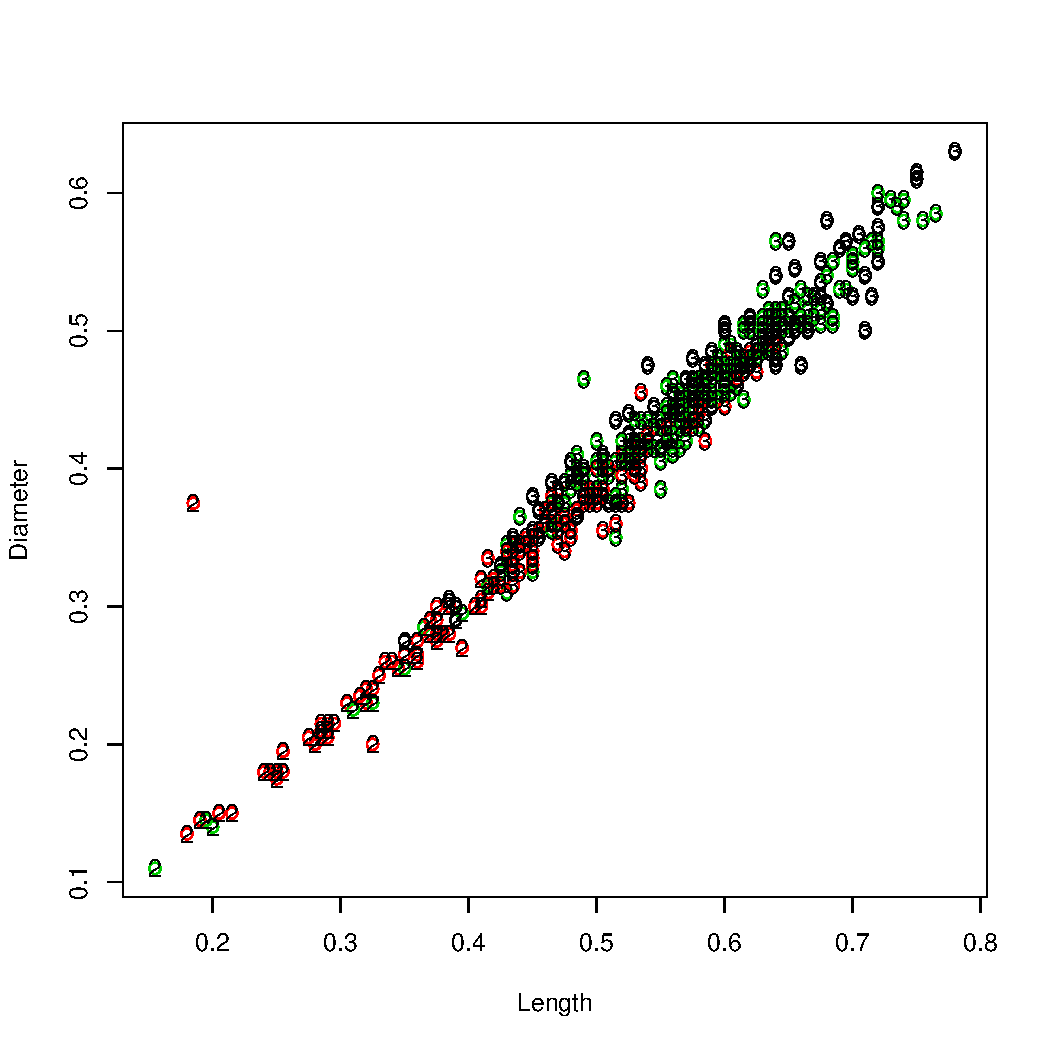
\includegraphics[width=\maxwidth]{figure/em_plot2-1} \caption[Classification of abalone based on length and diameter]{Classification of abalone based on length and diameter.  The algorithm used assumes the covariance matrix does not differ between the three categories.}\label{fig:em_plot2}
\end{figure}


\end{knitrout}

The classification using the second algorithm Figure~\ref{fig:em_plot2}.  Using this algorithm, the proportion of correct classifications is 0.484.



\section*{Question 4}
I built the R package and did the check.  The package is called 'rlasso\_1.0.tar.gz', and the output from the build and check commands can be found in the file 'q4\_buildcheck\_output.txt'.


\end{document}
